\section*{\hypertarget{job}{Jobs}}
\addcontentsline{toc}{subsection}{Jobs}
%
"Off my seat, Jester. The King sits there." \\
\indent -- Noctis 
%
\begin{center}

\includegraphics[width=\columnwidth]{./art/images/ff10-2.png} 
\end{center}
%
Your character's Job determines his or her combat proficiencies including abilities, attributes and equipment expertise.
A character's combat prowess increases further as he or she specializes in a job by gaining experience and Levels.
All available jobs are detailed in their \textbf{Job descriptions} right after this page.
We recommend that you print or copy the description of your chosen Job to use as the second page of your character sheet.
Your character's attributes initially all start at 0 and increase by progressing in a job.
The \textbf{Basic Attributes} table shows your character's attribute gains and equipment expertise at Level~1.
The \textbf{Abilities} table shows which spells and techniques your character learns at different Levels.

\subsubsection*{Archetype}
When your character reaches \textbf{Level~4} in his or her Job, you have to decide between one of its two Archetypes. 
Archetypes represent play styles within a job and can be regarded as taking different approaches to fulfil the same role.
They emphasize progress in different aspects of combat by supporting a character's abilities through passive benefits. 
At Level~4, the chosen archetype grants your character \hyperlink{sabilities}{Passive and Reaction} abilities and also determines the attribute progression at further Levels.
\pagebreak
\subsubsection*{Limit Break}
Starting at \textbf{Level 5} you can choose any of your character's known abilities to become their Limit Break, which is an enhanced version of the original ability.
You can only change the Limit Break to another ability during Level up and you can still use the chosen ability in its original version.
When you use the Limit Break ability, it costs twice the amount of MP as usual and gains \textbf{one of the following} additional effects of your choice:
\begin{itemize}[leftmargin=*]  
	\item The amount of damage dealt or HP restored by the original ability is doubled.
	\item If the original ability targets a single entity, you can target two entities within its range. If the ability targets an area, the target distance  is doubled.
	\item If the original ability has an effect that lasts for a duration, the duration is doubled.	
	\item If the original ability requires you or the target to pass a check, you can increase or decrease the DC by 2 depending on which benefits you.	
\end{itemize}

\vspace{0.7cm}

\subsubsection*{Job Change}
You can change your character's job only once during the adventure after reaching a Level up.
Instead of increasing the Level of his or her old job, your character starts at Level~1 in the new job.
When changing your character's job, he or she keeps all of the learned abilities, attribute improvements and equipment expertise from the old job.  
The only exception to this is the AGI attribute, where your character only gains the higher bonus between the two jobs.
However, your character can only have a total maximum of 10 Levels between both jobs.
Accordingly, the flexibility of changing jobs comes at the cost of not being able to become an expert in either one.
\vspace{1cm}
%
\example{Job Change}{
After fighting through the Wind Shrine and reaching its top, Bartz and his party realize that the Wind Crystal has already been destroyed.
Regardless, the GM awards the party with a Level Up and everyone in the party except Bartz advances from Level 2 to 3.
Bartz picks up one of the crystal shards and suddenly feels a rush of energy, which imbues him with magical powers.
Instead of leveling up, he changes his job into Black Mage, starting at Level 1.
Nevertheless, he keeps his attributes and the ability to equip swords and armor from his old Warrior job.
In addition, his attributes	are increased as noted in the job description for Level 1 Black Mages.
The only exception is the AGI attribute, which he keeps from its old job since it is higher.
Bartz also learns the spells "Fire", "Ice" and "Lightning" in addition to the "Rush" and "Beatdown" Techs that he already knows.
}
%
\pagebreak
%
\thispagestyle{empty}
\subsection*{\huge Black Mage}
\vspace{0.3cm}
"You sure are a keen observer of the obvious, kupo!" \\
\indent -- Montblanc 
\vspace{0.3cm} \\
Black magic is a pathway to many abilities some consider to be unnatural. 
Black Mages are fragile in physical combat, but can wipe out multiple enemies from great distances and inflict nasty status effects. 
They can thus assert great control over the battlefield and are difficult to ignore for enemies. \\
\vfill
\battrt
{
	\textbf{Level 1:} & HP~+17 & MP~+21 & AGI~+2 & MAG~+1  \\
	\textbf{Level 2:} & HP~+5  & MP~+10 & STR~+1 & RES~+1  \\
	\textbf{Level 3:} & HP~+10 & MP~+10 & MAG~+1 &         
}
{Staff}
{Robe}
\vfill
\atypet{Arcanist}
{
	\textbf{Level 4:} & HP~+5  & MP~+5  & MAG~+2 & DEF~+1 \\ 
	\textbf{Level 5:} & HP~+5  & MP~+10 & RES~+1 & MAG~+1 \\ 
	\textbf{Level 6:} & HP~+5  & MP~+10 & RES~+1 & DEF~+1 \\
	\textbf{Level 7:} & HP~+10 & MP~+10 & MAG~+1 &  	  \\
	\textbf{Level 8:} & HP~+5  & MP~+10 & MAG~+1 & DEF~+1 \\
	\textbf{Level 9:} & HP~+10 & MP~+5  & RES~+1 & MAG~+1 \\
	\textbf{Level 10:}& HP~+5  & MP~+10 & RES~+2 &		  
}
{Magic Boost}
{	
	Whenever you cast \hyperlink{action}{Magic} that targets a single entity, you can choose to also target everyone within 1u of him. The damage dealt to secondary targets is halved.
}
{Critical Vanish}
{	
	Whenever you have more than 1 HP and an \hyperlink{action}{Attack} would reduce you to 0 HP, you remain at 1 HP and gain \hyperlink{status}{Blink} for 3 rounds or until you take an action.
}
\vfill
\atypet{Scholar}
{	
	\textbf{Level 4:} & MP~+10 & RES~+1 & DEF~+1 & MAG~+1 \\
	\textbf{Level 5:} & HP~+10 & MP~+10 & MAG~+1 		  \\
	\textbf{Level 6:} & HP~+5  & MP~+10 & RES~+1 & MAG~+1 \\
	\textbf{Level 7:} & HP~+5  & MP~+10 & MAG~+2  		  \\
	\textbf{Level 8:} & HP~+5  & MP~+10 & RES~+1 & DEF~+1 \\
	\textbf{Level 9:} & HP~+5  & MP~+10 & RES~+1 & MAG~+1  \\
	\textbf{Level 10:}& HP~+10 & MP~+10 & MAG~+1		  \\
}
{Turbo MP}
{	
	Whenever you begin casting \hyperlink{action}{Magic}, you can choose to double its range by also doubling the MP cost.
}
{Return Magic}
{	
	Whenever you suffer damage caused by \hyperlink{action}{Magic}, you can cast the same spell back to its caster.
	In doing this, you have to respect the cast time and MP cost of the spell.
	If you are already casting another spell, you have to break its concentration to use this effect. 
}
\pagebreak \\
\noindent {\Large\color{accent}\bf \uline{Abilities\phantom{y}\hfill}}\\\\
\spellt{Fire}{4}{1r}{Single}{3u}
{
	You deal 2d \hyperlink{type}{fire} damage to the target.
}{\fire}{1}
\spellt{Blizzard}{4}{1r}{Single}{3u}
{
	You deal 2d \hyperlink{type}{ice} damage to the target.
}{\ice}{1}
\spellt{Thunder}{4}{1r}{Single}{3u}
{
	You deal 2d \hyperlink{type}{lightning} damage to the target.
}{\lightning}{1}
\spellt{Blind}{6}{1r}{Single}{3u}
{
	The target makes a DC 8 check and suffers \hyperlink{status}{Blind} for 3 rounds upon failure.
}{\blind}{2}
\spellt{Bio}{8}{1r}{Single}{3u}
{
	The target makes a DC 8 check and suffers 2d damage and \hyperlink{status}{Poison} for 3 rounds upon failure.
}{\poison}{3}
\spellt{Firaga}{12}{2r}{Single}{5u}
{
	You deal 6d \hyperlink{type}{fire} damage to the target. 
}{\fire}{5}
\spellt{Blizzaga}{12}{2r}{Single}{5u}
{
	You deal 6d \hyperlink{type}{ice} damage to the target. 
}{\ice}{5}
\spellt{Thundaga}{12}{2r}{Single}{5u}
{
	You deal 6d \hyperlink{type}{lightning} damage to the target. 
}{\lightning}{5}
\spellt{Rasp}{4}{1r}{Single}{5u}
{
	You reduce the target's MP by 4d.
}{}{6}
\spellt{Quake}{22}{2r}{3u}{8u}
{
	Deal 8d \hyperlink{type}{earth} damage to everyone in the target area. 
}{\earth}{7}
\spellt{Flare}{24}{3r}{Single}{5u}
{
	You deal 9d+15 \hyperlink{type}{fire} damage to the target. 
}{\fire}{8}
\spellt{Doom}{28}{1r}{Single}{5u}
{
	The target makes a DC 8 check and suffers \hyperlink{status}{KO} after 3 rounds upon failure.
}{\ko}{9}
\spellt{Ultima}{40}{3r}{3u}{5u}
{
	Deal 10d+20 \hyperlink{type}{dark} damage to all enemies in the target area. 
}{\dark}{10}
\pagebreak
\ofjob{Dragoon}
{
	\ofquote{"Confident bastard, aren't you?"\\}{Kain}\\\\
	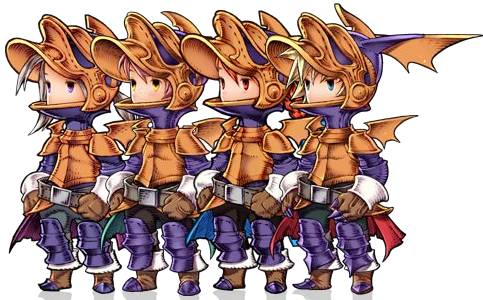
\includegraphics[width=\columnwidth]{./art/jobs/dragoon.jpg}\ofrow
	\accf{Dragoons} are masters of aerial combat, who strike their enemies with devastating attacks from the sky.
	They prefer spears as their weapon and have an affinity for the fire element. 
	Even though they are humanoid, it is said that Dragoons have the soul of a dragon.
}
{Spear}{Heavy Armor}{
	Level 1: & HP +23 & MP~+16 & AGI~+2,& STR~+1 \\
	Level 2: & HP~+10  & MP~+5 & STR~+1 & RES~+1 \\
	Level 3: & \multicolumn{3}{l}{Archetype Attribute Bonus} \\
	Level 4: & HP~+5  & MP~+10 & DEF~+2 &  	  \\
	Level 5: & HP~+10 & MP~+10 & STR~+1 & 		  \\ 
	Level 6: & HP~+10 & MP~+10 & RES~+1 		  \\
	Level 7: & HP~+10 & MP~+5  & STR~+1 & 	DEF~+1	  \\ 
	Level 8: & HP~+10 & MP~+10 & RES~+1 & 	 	  \\ 
	Level 9: & HP~+10  & MP~+10 & STR~+1 \\ 
	Level 10:& HP~+10  & RES~+1 & DEF~+2 
}{
	\ofjobtech{Jump}{3}{1r}{Single}{3u}{When you begin using this Tech, you jump 3u up into the air. After the cast time is up, you leap onto the target and make an Attack on him.}{}{1}\ofabilitygap
	\ofjobtech{Lancet}{3}{0r}{Single}{5u}{You deal damage to the target's HP and MP by an amount equal to your current Level and increase your own HP and MP by the same amount. This amount is not recued by the target's DEF or RES.}{}{2}\ofabilitygap
	\ofjobtech{Double Jump}{8}{1r}{Single}{3u}{When you begin using this tech, you jump 3u up into the air. After the cast time is up, you leap onto the target and make an Attack on him. You can then leap to another location within 3u. If you land on another enemy you can make an Attack on him too.}{}{6}\ofabilitygap
	\ofjobtech{Roar}{8}{0r}{5u}{Self}{All enemies in the target area make a DC 9 check and suffer 2d damage and Immobile for 1 round upon failure.}{\immobile}{8}\ofabilitygap
	\ofjobtech{Highwind}{24}{1r}{Single}{Self}{For the next 3 rounds, you stay up to 3u in the air from where you can move your usual distance and perform one of the following 2 actions without additional MP cost or cast time on each turn:\\ 
		\acc{Lance Barrage:} make an Attack against a target within 10u. If you hit, you score a Critical Hit.\\
		\acc{Fire Blast:} choose a target within 10u. He and all enemies within 2u of him suffer 4d fire damage.
	}{\fire}{10}
}{
	\ofarchetypet{Dragon Knight}
	{HP~+8 & MP~+12 & STR~+1 & RES~+2}
	{\ofarchetypetecha{Fire Breath}{7}{0r}{3u (front)}{Self}{You deal 2d fire damage to everyone in the target area.}{\fire}}
	{\ofarchetypepassive{Flametongue}{You gain permanent Resilience against fire damage. Furthermore, whenever you deal physical damage to an enemy, you can choose to let the damage dealt be of magical and fire type instead.}}
	{\ofarchetypereaction{Dragonheart}{Whenever you deal or receive fire damage, you gain EnSTR until the end of your next turn.}}
	{\ofarchetypetechb{Dragon Dive}{16}{1r}{3u}{7u}{When you begin using this Tech, you jump 3u up into the air. After the cast time is up you leap onto the target and deal 4d fire damage to everyone in the target area except yourself. Also, you create Hot Field in the target area that lasts for 3 rounds but does not affect you.}{\fire}}
}{
	\ofarchetypet{Valkyrie}
	{HP~+13 & MP~+7 & STR~+2 & DEF~+1}
	{\ofarchetypetecha{Full Thrust}{6}{0r}{5u (line)}{Self}{You dash forward in an up to 5u long line. Make an Attack on everyone in the way by making one damage roll that is applied to all targets that fail to evade.}{}}
	{\ofarchetypepassive{Duelist}{As long as you are in combat within 3u of one enemy and there is noone else within 3u of you, the STR bonus added to your Attacks and Abilities is doubled.}}
	{\ofarchetypereaction{Arm's Length}{Whenever an enemy walks within 2u of you, he has to make a DC~7 check and upon failure he cannot move any further towards you on this turn.}}
	{\ofarchetypetechb{Revenge}{12}{0r}{Single}{Weapon}{Make an Attack on an enemy that has damaged you since your last turn. On hit, you inflict the damage that he dealt to you before instead of your usual damage.}{}}
}
\ofjob{Marksman}
{
	\ofquote{"I play the leading man; who else?"\\}{Balthier}\\\\
	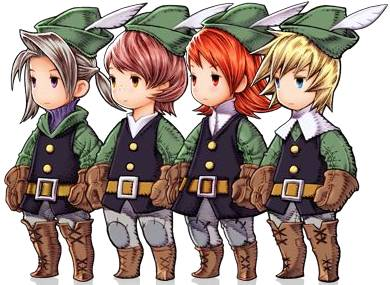
\includegraphics[width=\columnwidth]{./art/jobs/marksman.jpg}\ofrow
	\accf{Marksmen} are experts of all kinds of ranged weapons that strike from great distance. 
	Skilled Marksmen can see through their enemies, allowing them to know a target's strengths and weaknesses. 
	Therefore they can not only deal significant ranged damage, but also disable enemies with special techniques.
}
{Bow or Gun}{Light Armor}{
	Level 1: & HP +19 & MP~+17 & AGI~+2 & STR +1 \\
	Level 2: & HP~+10  & MP~+10 & DEF~+1 \\
	Level 3: & \multicolumn{3}{l}{Archetype Attribute Bonus}  \\
	Level 4: & HP~+5  & MP~+5  & STR~+2 & RES~+1 \\
	Level 5: & HP~+5  & MP~+10 & DEF~+1 & RES~+1  \\
	Level 6: & HP~+10 & MP~+10 & RES~+1 &        \\
	Level 7: & HP~+5  & MP~+10 & STR~+1 & RES~+1 \\
	Level 8: & HP~+10  & MP~+5 & DEF~+2 		  \\
	Level 9: & HP~+5  & MP~+10 & RES~+1 & STR~+1 \\
	Level 10:& HP~+10 & MP~+10 & STR~+1 &        
}{
	\ofjobtech{Libra}{4}{0r}{Single}{5u}{You analyse the target thoroughly and know his Resiliences, Weaknesses, Immunities, as well as his current HP and MP.}{}{1}\ofabilitygap
	\ofjobtech{Heavy Shot}{6}{0r}{Single}{Weapon}{Make an Attack on the target. If you hit, the damage dealt ignores the target's DEF.}{}{2}\ofabilitygap
	\ofjobtech{Fast Draw}{8}{0r}{Single}{Weapon}{You make an Attack after which you can immediately begin using another Ability in the same turn.}{}{4}\ofabilitygap
	\ofjobtech{Explosive Shot}{10}{0r}{2u}{Weapon}{Everyone in the target area suffers 3d fire damage. In addition, you create a Hot Field in the target area that lasts for 3 rounds.}{\fire}{6}\ofabilitygap
	\ofjobtech{Smoke Bomb}{10}{0r}{3u}{10u}{You create an Obscure Field in the target area that lasts for 3 rounds.}{}{8}\ofabilitygap
	\ofjobtech{Barrage}{22}{1r}{Single}{Self}{You gain Haste and EnSTR for 3 rounds. Also, all your Attacks and Techs which target a single enemy instead affect all enemies within 2u of the chosen target.
	}{\haste\enstr}{10}
}{
	\ofarchetypet{Ranger}
	{HP~+13 & MP~+12 & DEF~+2}
	{\ofarchetypetecha{Lay Trap}{4}{0r}{1u}{Self}{You set a trap where you are standing. An enemy that walks over it makes a DC 9 check and suffers 1d damage and Immobile for 1 round upon failure. The trap disappears once it is activated.}{\immobile}}
	{\ofarchetypepassive{Recoil}{Whenever you make a successful Attack, you can immediately move 1u in any direction.}}
	{\ofarchetypereaction{Magic Evade}{You can evade Magic by passing an evasion check. When you evade an Attack or Magic, you also regain an amount of MP equal to your current Level.}}
	{\ofarchetypetechb{Poison Ammo}{10}{0r}{Single}{Weapon}{Make an Attack on the target. If you hit, the damage dealt is magical and the target makes a DC 8 check. Upon failure, he suffers Poison, DeSTR and DeDEF for 3 rounds.}{\poison\destr\dedef}}
}{
	\ofarchetypet{Sniper}
	{HP~+5 & MP~+15 & STR~+3}
	{\ofarchetypetecha{Pierceshot}{6}{0r}{10u (line)}{Self}{Make an Attack against all targets in a line, by making one damage roll that applies to everyone that fails to evade.}{}}
	{\ofarchetypepassive{Concentrate}{Whenever you Attack an enemy, he has Disadvantage on the evasion check.}}
	{\ofarchetypereaction{Camouflage}{Whenever you end a turn in which you have not moved, you gain Blink until the start of your next turn.}}
	{\ofarchetypetechb{Aim}{8}{0r}{Single}{Weapon}{Make an Attack on the target and choose one of the following spots to inflict an additional effect if you hit:\\ \acc{Head:} the target's evasion DC is reduced by 2, but if you hit you score a Critical Hit.\\ \acc{Heart:} MP is reduced by same amount as HP.\\ \acc{Leg:} the target suffers Immobile for 1 round.}{\immobile}}
}
\ofjob{Monk}
{
	\ofquote{"Now I know why I have these stupid muscles!"\\}{Sabin}\\\\
	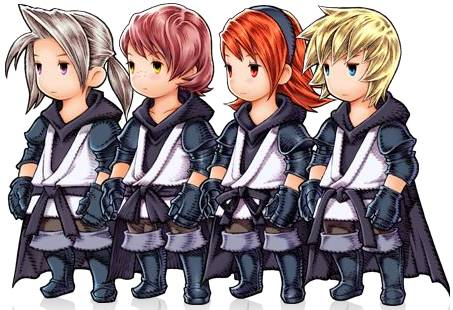
\includegraphics[width=\columnwidth]{./art/jobs/monk2.jpg}\ofrow
	\accf{Monks} are adept melee fighters that posses a deadly combination of strength and technique.
	While they do not have expertise in using magic, Monks can produce similarly incredible effects by tapping into their inner life force. 
	A skilled monk absorbs what is useful, discards what is useless and adds what is specifically his own.
}
{None}{Light Armor}{
	Level 1: & HP +20 & MP~+13 & AGI~+4 & \\
	Level 2: & HP~+10 & MP~+5  & STR~+2 & \\
	Level 3: & \multicolumn{3}{l}{Archetype Attribute Bonus} \\
	Level 4: & HP~+5  & MP~+10 & STR~+1 & RES~+1 \\
	Level 5: & HP~+10  & MP~+5 & DEF~+1 & STR~+1 \\
	Level 6: & HP~+10 & MP~+5  & STR~+1 & RES~+1 \\
	Level 7: & HP~+10 & MP~+5  & STR~+1 & DEF~+1 \\ 
	Level 8: & HP~+10 & MP~+5  & DEF~+2 &        \\
	Level 9: & HP~+5  & MP~+10 & STR~+1 & RES~+1 \\ 
	Level 10: & HP~+10 & MP~+10 & DEF~+1 &        \\ 
}{
	\ofjobpassive{Brawler}{In combat, you can use your bare fists as your weapon. They have the same DMG as weapons of the highest equipment class that you can use. Also, you can carry a third Accessory in place of your weapon slot and you gain STR +1 for every equipped Accessory.}{1}\ofabilitygap
	\ofjobtech{Kick}{4}{0r}{1u}{Self}{You make an Attack against all enemies within 1u of you, by making one damage roll that applies to all affected targets that fail to evade. All targets that fail to evade are also knocked back by 1u.}{}{2}\ofabilitygap
	\ofjobtech{Aurablast}{6}{0r}{Single}{3u}{You deal an amount of magical damage equal to your current Level to the target.}{}{4}\ofabilitygap
	\ofjobtech{Pummel}{8}{0r}{Single}{1u}{You make 2 consecutive Attacks against the target.}{}{6}\ofabilitygap
	\ofjobtech{Blitz}{3}{0r}{Single}{Self}{You use two different Techs consecutively in the same turn. In doing this, you have to respect additional MP costs and cast times of both Techs.}{}{8}\ofabilitygap
	\ofjobtech{Final Heaven}{22}{0r}{Single}{1u}{You deal 6d damage to the target and knock him back by 5u. If he hits a wall or a similarly solid object in doing so, you deal another 3d damage to him.}{}{10}
}{
	\ofarchetypet{Black Belt}
	{HP~+17 & MP~+8 & STR~+2}
	{\ofarchetypetecha{Bonecrusher}{6}{0r}{Single}{1u}{Make an Attack against the target. If you hit, the target makes a DC~8 check and suffers Slow for 1 round upon failure.}{}}
	{\ofarchetypepassive{Unscarred}{As long as your current HP is equal to your maximum HP, the STR bonus that is added to the damage dealt by your Attacks is doubled.}}
	{\ofarchetypereaction{Strikeback}{Whenever you successfully evade an Attack by an enemy, you immediately make an Attack on him, if he is within range.}}
	{\ofarchetypetechb{Meteor Strike}{14}{0r}{Single}{1u}{You slam the target into the ground dealing 5d damage. In doing this, you can also leap to a location of your choice within 3u.}{}}
}{
	\ofarchetypet{Templar}
	{HP~+4 & MP~+16 & DEF~+1 & RES~+2}
	{\ofarchetypetecha{Chakra}{6}{1r}{Single}{Self}{You regain an amount of HP equal to your current Level and recover from one Status Effect that you are currently suffering.}{}}
	{\ofarchetypepassive{Lifestream}{If you do not have enough MP to use an ability you can instead choose to reduce your HP by the amount of its MP cost in order to use it.}}
	{\ofarchetypereaction{Replenish MP}{Whenever you suffer physical damage, you regain an amount of MP equal to half your current Level.}}
	{\ofarchetypetechb{Revive}{14}{1r}{Single}{1u}{You remove KO from the target and increase his HP by~1.}{\ko}}
}
\ofjob{Red Mage}
{
	\ofquote{"Oh, I’ll show you how lightning strikes."\\}{Lightning}\\\\
	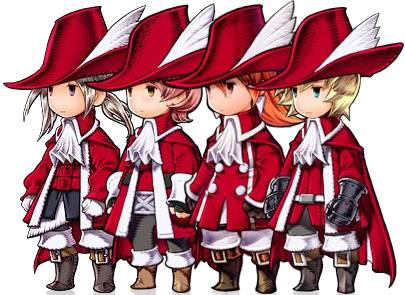
\includegraphics[width=\columnwidth]{./art/jobs/redmage.jpg}\ofrow
	\accf{Red Mages} are very versatile and possess a wide variety of abilities, but can also hold their own in melee combat. 
	Although they excel in neither discipline, Red Mages are still a force to be reckoned with.
}
{Rod or Sword}{Light Armor or Robe}{
	Level 1: & HP~+20 & MP~+21 & AGI~+3 & STR +1 \\
	Level 2: & HP~+5  & MP~+10 & MAG~+1 & DEF~+1 \\
	Level 3: & \multicolumn{3}{l}{Archetype Attribute Bonus}   \\
	Level 4: & HP~+10 & MP~+5  & STR~+1 & RES~+1 \\   
	Level 5: & HP~+5  & MP~+10 & MAG~+2 & 		  \\ 
	Level 6: & HP~+5 & MP~+10  & STR~+1 &	MAG~+1 \\ 
	Level 7: & HP~+10  & MP~+10 & DEF~+1 \\ 
	Level 8: & HP~+10 & MP~+5  & STR~+1 & MAG~+1 \\ 
	Level 9: & HP~+5  & MP~+10 & RES~+2 \\ 
	Level 10: & HP~+10 & MP~+10 & STR~+1 		  
}{	
	\ofjobspell{Cure}{4}{0r}{Single}{3u}{The target regains 2d HP.}{}{1}\ofabilitygap
	\ofjobspell{Fire}{4}{0r}{Single}{3u}{You deal 2d fire damage to the target.}{\fire}{2}\ofabilitygap
	\ofjobspell{Blizzard}{4}{0r}{Single}{3u}{You deal 2d ice damage to the target.}{\ice}{2}\ofabilitygap
	\ofjobspell{Thunder}{4}{0r}{Single}{3u}{You deal 2d lightning damage to the target.}{\lightning}{2}\ofabilitygap
	\ofjobspell{Blind}{6}{0r}{Single}{5u}{The target makes a DC~8 check and suffers Blind for 3 rounds upon failure.}{\blind}{4}\ofabilitygap	
	\ofjobspell{Esuna}{6}{0r}{Single}{3u}{You remove all negative Status Effects except KO from the target.}{}{6}\ofabilitygap
	\ofjobspell{NulElement}{10}{0r}{Single}{5u}{Choose an element (e.g. fire). The target does not suffer any damage of the chosen element for 3 rounds.}{}{8}\ofabilitygap
	\ofjobspell{Dualcast}{4}{0r}{Single}{Self}{You begin casting and concentrating on two spells of your choice simultaneously, but need to spend the necessary MP for both.}{}{10}
}{
	\ofarchetypet{Ravager}
	{HP~+6 & MP~+14 & MAG~+2 & RES~+1}
	{\ofarchetypespella{Poison}{6}{0r}{Single}{5u}{The target makes a DC~8 check and suffers Poison for 3 rounds upon failure.}{\poison}}
	{\ofarchetypepassive{Stagger}{Whenever you inflict one or more Status Effects on an enemy, he additionally suffers an amount of magical damage equal to your MAG.}}
	{\ofarchetypereaction{Swiftcast}{When you suffer damage from an enemy, you can immediately use an ability on him if he is within range.}}
	{\ofarchetypespellb{Imperil}{8}{0r}{Single}{5u}{The target suffers DeDEF and DeRES for 3 rounds.}{\dedef \deres} \ofabilitygap \ofarchetypespellb{Wall}{8}{0r}{Single}{5u}{The target gains EnDEF and EnRES for 3 rounds.}{\enndef \enres}}
}{
	\ofarchetypet{Spellblade}
	{HP~+14 & MP~+6 & STR~+2 & DEF~+1}
	{\ofarchetypetecha{Elemental Strike}{4}{0r}{Single}{Weapon}{Choose an element (e.g. fire) and make an Attack. If you hit, the damage is of magical type with the chosen element and you also add your MAG to the damage dealt.}{}}
	{\ofarchetypepassive{Magic Weapon}{Whenever you cast Magic, you can choose to store the spell inside your weapon. In this case, the spell's MP cost is halved. All stored spells take effect together with your next successful Attack and you can chose targets within their range including yourself. You cannot store more than two spells at once inside your weapon.}}
	{\ofarchetypereaction{Mana Shield}{Whenever your HP is reduced, you can instead choose to reduce your MP by the same amount.}}
	{\ofarchetypetechb{Phantom Blade}{5}{0r}{Single}{5u}{Make an Attack on a target within range as if you were standing next to him. This Attack cannot be evaded.}{}}
}
\ofjob{Sentinel}
{
	\ofquote{"Allow me to shatter your delusions of grandeur."\\}{Beatrix}\\\\
	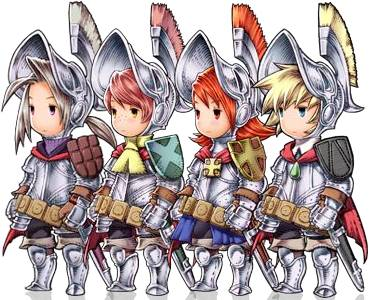
\includegraphics[width=\columnwidth]{./art/jobs/sentinel.jpg}\ofrow
	\accf{Sentinels} are masters of defensive combat who will rarely fall in a battle.  
	Their special abilities allow them to not only withstand incredible amounts of damage, but also provide protection to their allies.
	A capable Sentinel is often the last thing standing between the party and certain death.
}
{Sword}{Heavy Armor}{
	Level 1: & HP~+27 & MP~+18 & AGI~+3 & DEF~+1  \\
	Level 2: & HP~+10 & MP~+10 & STR~+1 & RES~+1 \\
	Level 3: & \multicolumn{3}{l}{Archetype Attribute Bonus} \\
	Level 4: & HP~+10 & MP~+5  &  DEF~+1 & STR~+1 \\ 
	Level 5: & HP~+10 & MP~+5  & RES~+1 & DEF~+1 \\ 
	Level 6: & HP~+10 & MP~+10 & STR +1 &        \\
	Level 7: & HP~+10 & MP~+5  & DEF +2 &        \\
	Level 8: & HP~+10 & MP~+5  & STR +1 & DEF~+1 \\
	Level 9: & HP~+10 & MP~+10 & STR +1 &        \\
	Level 10: & HP~+10  & MP~+10 & DEF +1 
}{
	\ofjobtech{Guard}{3}{0r}{Single}{Self}{You gain EnDEF until the end of your next turn.}{\enndef}{1}\ofabilitygap
	\ofjobtech{First Aid}{5}{0r}{Single}{1u}{Choose a target that has received damage since your last turn, including yourself. The target regains 2d HP.}{}{2}\ofabilitygap
	\ofjobtech{Mediguard}{10}{0r}{Single}{Self}{You gain EnDEF and Regen for 3 rounds.}{\enndef}{6}\ofabilitygap
	\ofjobtech{Barrier}{10}{0r}{3u}{Self}{You and all allies within the target area gain Blink for 2 rounds.}{\blink}{8}\ofabilitygap
	\ofjobtech{Vengeance}{14}{0r}{Single}{1u}{Make an Attack against the target. If you hit, the target suffers the difference between your current and your maximum HP instead of your usual damage.}{}{8}\ofabilitygap
	\ofjobtech{Mighty Guard}{26}{1r}{Single}{Self}{For the next 3 rounds, you gain Resilience against all physical and magical damage.}{}{10}
}{
	\ofarchetypet{Defender}
	{HP~+17 & MP~+3 & STR~+2 & DEF~+1}
	{\ofarchetypetecha{Powerbreak}{6}{0r}{Single}{1u}{Make an Attack on the target.  If you hit, he suffers DeSTR and DeMAG for 3 rounds on top of the damage dealt.}{\destr \demag}}
	{\ofarchetypepassive{Provoke}{Whenever you successfully Attack an enemy, you can try to provoke him. If you do so, he has to make a DC~8 check and upon failure he has to target you with an action on his next turn if possible.}}
	{\ofarchetypereaction{Block}{Whenever an enemy within 2u of you tries to move away from you, he has make a DC 8 check. Upon failure, he suffers Immobile until the start of his next turn, preventing him from moving any further on this turn.}}
	{\ofarchetypetechb{Threaten}{8}{0r}{Single}{5u}{The target makes a DC 8 check and suffers 2d damage and Immobile for 3 rounds upon failure.}{\immobile}}
}{
	\ofarchetypet{Paladin}
	{HP~+10 & MP~+15 & RES~+2}
	{\ofarchetypetecha{Earth Wall}{8}{0r}{3u (line)}{8u}{You create a 3u tall and wide wall of earth that blocks the path. The wall breaks down after 3 rounds or upon suffering a total of 15 damage. You cannot use this ability if a previous wall still exists.}{}}
	{\ofarchetypepassive{Holy Guard}{As long as there is at least one ally within 1u of you, you and all allies within 1u gain EnRES.}}
	{\ofarchetypereaction{Cover}{Whenever an ally within 1u of you receives physical damage, you can decide to direct half of the total damage dealt on yourself instead of onto your ally.}}
	{\ofarchetypetechb{Astra}{8}{0r}{Single}{5u}{For the next 5 rounds, the target becomes Immune to all Status Effects.}{}}
}

\thispagestyle{empty}
\subsection*{\huge Invocador}
\vspace{0.3cm}
"No me gusta tu plan. Apesta." \\
\indent -- Yuna 
\vspace{0.3cm} \\
Los Invocadores son poderosos hechiceros que pueden invocar bestias mágicas para que los asistan en combate. Crean un fuerte vínculo con su invocación, que permite al Invocador controlar sus increíbles poderes a voluntad. Aunque los Invocadores se centran en usar magia defensiva, sus invocaciones pueden causar más estragos que cualquier ser humano.
\vfill
\battrt{ \textbf{Nivel 1:} & PV~+16 & PM~+19 & AGI~+2 & MAG~+1 \\ 
 \textbf{Nivel 2:} & PV~+5 & PM~+10 & RES~+1 & FUE~+1 \\ 
 \textbf{Nivel 3:} & PV~+10 & PM~+10 & MAG~+1 &         
}{Bastón}{Túnica}
\vfill
\atypet{Devoto} { \textbf{Nivel 4:} & PV~+5 & PM~+10 & RES~+1 & DEF~+1 \\  
 \textbf{Nivel 5:} & PV~+10 & PM~+10 & MAG~+1 &        \\  
 \textbf{Nivel 6:} & PV~+5 & PM~+10 & MAG~+1 & RES~+1 \\  
 \textbf{Nivel 7:} & PV~+5 & PM~+10 & RES~+2 &        \\  
 \textbf{Nivel 8:} & PV~+10 & PM~+10 & DEF~+1 &		  \\  
 \textbf{Nivel 9:} & PV~+5 & PM~+10 & MAG~+1 & RES~+1 \\  
 \textbf{Nivel 10:}& PV~+10 & PM~+10 & MAG~+1 &        \\  
} {Unión de Almas} { En tu turno, la invocación que esté activa puede lanzar un hechizo utilizando tus PM además de los suyos y el tiempo de lanzamiento del hechizo se reduce en 1 turno. Debes omitir tu propio turno para utilizar este efecto. } {Sacrificio} { Siempre que tu invocación activa reciba algún daño, puedes elegir reducir tus propios PV en su lugar. }
\vfill
\atypet{Evocador} { \textbf{Nivel 4:} & PV~+10 & PM~+5 & MAG~+1 & DEF~+1 \\  
 \textbf{Nivel 5:} & PV~+10 & PM~+10 & RES~+1 &		  \\  
 \textbf{Nivel 6:} & PV~+5 & PM~+10 & MAG~+1 & RES~+1 \\  
 \textbf{Nivel 7:} & PV~+10 & PM~+5 & DEF~+1 & RES~+1 \\  
 \textbf{Nivel 8:} & PV~+5 & PM~+10 & MAG~+2 &	      \\  
 \textbf{Nivel 9:} & PV~+5 & PM~+10 & RES~+1 & MAG~+1 \\  
 \textbf{Nivel 10:}& PV~+10 & PM~+10 & RES~+1 &		  \\  
} {Canalizar} {En tu turno, puedes elegir lanzar un hechizo de tu invocación activa. El tiempo de lanzamiento del hechizo se reduce en 1 turno. La invocación debe omitir su turno para poder utilizar este efecto. } {Lazo Vital} { Siempre que recibas algún daño, puedes elegir reducir los PV de tu invocación activa en vez de los tuyos. }
\pagebreak \\
\noindent {\Large\color{accent}\bf \uline{Habilidades\phantom{y}\hfill}}\\\\
\spellt{Invocar}{8}{3t}{Único}{Tú} { Invocas a una criatura que actúa junto a ti en tu turno siguiendo tus instrucciones. La invocación desaparece cuando tú o la invocación pasen a estar \hyperlink{status}{KO}, pero también puedes cancelarla cuando desees. Una vez que la invocación sea cancelada o derrotada, no podrás volver a invocar a la misma criatura en ese mismo día. Todas las criaturas que puedes invocar en tus diferentes niveles de personaje se muestran en la página siguiente. }{}{1} \spellt{Plegaria}{5}{1t}{1u}{Tú}{ Todos los que se encuentren en el área de efecto recuperan 1d de PV. }{}{2} \spellt{Imagen}{10}{1t}{1u}{3u}{ El objetivo obtiene \hyperlink{status}{Reflejos} por 3 turnos. }{\blink}{4} \spellt{Rana}{16}{1t}{Único}{3u}{ El objetivo debe hacer una tirada con DC 8. Si falla, queda convertido en una rana por 3 turnos o hasta que reciba daño. Mientras esté convertido en rana, el objetivo no puede hablar ni realizar ninguna acción y solo puede moverse 1u por turno. }{}{6} \spellt{Disipar}{20}{1t}{Único}{3u}{ Eliminas todas las \hyperlink{type}{Resistencias} e \hyperlink{status}{Inmunidades} del objetivo por 3 turnos. Además, se eliminan todos los \hyperlink{status}{Estados Alterados} beneficiosos que estén activos en el objetivo cuando este hechizo tenga efecto. }{}{8} \spellt{Invocación Gemela}{28}{5t}{Único}{Tú}{ Invocas a dos criaturas que actúan junto a ti en tu turno siguiendo tus instrucciones. Las invocaciones desaparecen cuando tú o las invocaciones pasen a estar \hyperlink{status}{KO}, pero también puedes cancelarla cuando desees. Una vez que la invocación sea cancelada o derrotada, no podrás volver a invocar a la misma criatura en ese mismo día. Todas las criaturas que puedes invocar en tus diferentes niveles de personaje se muestran en la página siguiente. }{}{10}
\vspace{5cm}
\pagebreak
\onecolumn
\noindent{\LARGE\color{accent}\bf \uline{Invocaciones\hfill} \\} \\
\thispagestyle{empty}

\begin{multicols}{2}
\friendly{Carbuncle}{1}{
\includegraphics[width=0.18\textwidth]{./art/monsters/carbuncle.png}}
{ PV: & \hfill 20 & PM: & \hfill 36\\
 FUE: & \hfill 1 & DEF: & \hfill 0 \\
 MAG: & \hfill 2 & RES: & \hfill 2 \\
 AGI: & \hfill 3 & Tamaño: & \hfill P\\
} { \textbf{Tacleo}: 1d de daño\phantom{y} \mspell{Espejo}{12}{1t}{Único}{3u}{El objetivo recibe un escudo mágico que hace rebotar el próximo hechizo que le lancen y se lo devuelve al lanzador.}{} }
\vspace{0.5cm} 
\friendly{Ifrit}{3}{
\includegraphics[width=0.23\textwidth]{./art/monsters/ifrit.png}}
{ PV: & \hfill 50 & PM: & \hfill 36\\
 FUE: & \hfill 2 & DEF: & \hfill 3 \\
 MAG: & \hfill 1 & RES: & \hfill 0 \\
 AGI: & \hfill 3 & Tamaño: & \hfill M\\
} { \textbf{Garra}: 2d de daño \\
 \textbf{Resistencia}:\fire \hfill \textbf{Debilidad:}\ice \mspell{Piro}{4}{1t}{Único}{3u}{Infliges 2d de daño de \hyperlink{fire}{Fuego} al objetivo.}{\fire} \mtech{Fuego Infernal}{12}{1t}{2u}{Tú}{Infliges 4d de daño de \hyperlink{type}{Fuego} a todos los que se encuentren en el área de efecto excepto a ti.}{\fire} }
\vspace{0.5cm} 
\friendly{Shiva}{5}{
\includegraphics[width=0.18\textwidth]{./art/monsters/shiva.png}}
{ PV: & \hfill 60 & PM: & \hfill 80\\
 FUE: & \hfill 1 & DEF: & \hfill 1 \\
 MAG: & \hfill 5 & RES: & \hfill 4 \\
 AGI: & \hfill 3 & Tamaño: & \hfill M\\
} { \textbf{Témpano}: 2d de daño, 3u de alcance \\
 \textbf{Resistencia}:\ice \hspace*{\fill} \textbf{Debilidad:}\fire \mspell{AntiEscudo}{5}{1t}{Único}{3u}{El objetivo sufre \hyperlink{status}{disDEF} por 3 turnos.}{\dedef} \mspell{AntiCoraza}{5}{1t}{Único}{3u}{El objetivo sufre \hyperlink{status}{disRES} por 3 turnos.}{\deres} \mtech{Muro de Hielo}{10}{1t}{3u (línea)}{3u}{ Creas un muro de hielo de 3u de alto y ancho que bloquea el paso por 5 turnos. El muro se rompe después de 5 turnos o tras sufrir un total de 30 puntos de daño. }{} \mspell{Polvo de Diamante}{20}{1t}{3u (frente)}{Tú}{ Todos los enemigos en el área de efecto reciben 6d de daño de \hyperlink{type}{Hielo} y quedan \hyperlink{status}{Inmóviles} por 1 turno. }{\ice\immobile} } \friendly{Fénix}{7}{
\includegraphics[width=0.2\textwidth]{./art/monsters/phoenix.png}}
{ PV: & \hfill 70 & PM: & \hfill 90\\
 FUE: & \hfill 0 & DEF: & \hfill 2 \\
 MAG: & \hfill 6 & RES: & \hfill 8 \\
 AGI: & \hfill 2 & Tamaño: & \hfill M\\
} { \textbf{Picotazo}: 1d de daño \\ 
 \textbf{Inmune}: \hyperlink{status}{Todos los Estados Alterados} \hfill \newline\textbf{Resistencia:}\fire\holy \mspell{Escudo}{5}{1t}{Único}{3u}{El objetivo recibe \hyperlink{status}{aumDEF} por 3 turnos.}{\enndef} \mspell{Coraza}{5}{1t}{Único}{3u}{El objetivo recibe \hyperlink{status}{aumRES} por 3 turnos.}{\enres} \mspell{Cura++}{18}{1t}{1u}{3u}{Todos los que se encuentren en el área de efecto recuperan 6d PV.}{} \mspell{Lázaro+}{28}{3t}{Único}{3u}{Elimina el estado \hyperlink{status}{KO} del objetivo y recupera completamente sus PV.}{\ko} }
\vspace{0.5cm} 
\friendly{Bahamut}{9}{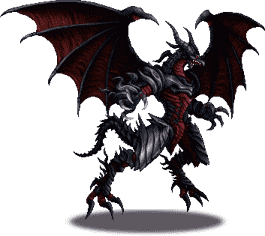
\includegraphics[width=0.23\textwidth]{./art/monsters/bahamut.png}}
{ PV: & \hfill 100 & PM: & \hfill 140\\
 FUE: & \hfill 8 & DEF: & \hfill 6 \\
 MAG: & \hfill 7 & RES: & \hfill 4 \\
 AGI: & \hfill 4 & Tamaño: & \hfill G\\
} { \textbf{Garra}: 3d de daño, 2u de alcance \\
 \textbf{Inmune}: \hyperlink{status}{Todos los Estados Alterados} \hfill \textbf{Resistencia:}\dark \mtech{Aliento Destructor}{20}{1t}{3u (frente)}{3u}{ Todos los que se encuentren en el área de efecto deben hacer una tirada con DC 8. Si fallan, reciben 4d de daño. Además, quedan \hyperlink{status}{Envenenados} y \hyperlink{status}{Ciegos} por 3 turnos. }{\poison \blind} \mspell{Desterrar}{30}{1t}{Único}{3u}{ El objetivo hace una tirada con DC 8. Si falla, es desterrado a otra dimensión, desapareciendo del campo de batalla por 3 turnos. }{} \mspell{Megafulgor}{40}{3t}{Único}{8u}{ Infliges 10d+20 de daño de \hyperlink{type}{Fuego} al objetivo. }{\fire} \mreaction{Ataque Final}{Si tus PV están a punto de llegar a 0, puedes usar una de tus habilidades sin costo ni tiempo de preparación antes de quedar \hyperlink{status}{KO}.} }
\end{multicols}
\twocolumn
\thispagestyle{empty}
\subsection*{\huge Thief}
\vspace{0.3cm}
"I PREFER the term ”treasure hunter!" \\
\indent -- Locke 
\vspace{0.3cm} \\
Thieves are extremely mobile melee fighters, who can quickly traverse the battlefield and are difficult
to hit with physical attacks. 
They excel at "borrowing" items and money from enemies and have a heightened sense for worthwhile business. 
One would be advised to be careful when dealing with a Thief, they always have one more trick up their
sleeve than you would expect.
\vfill
\battrt
{
	\textbf{Level 1:} & HP +20 & MP~+14 & AGI~+4 &        \\
	\textbf{Level 2:} & HP~+5  & MP~+5  & STR~+2 & DEF~+1 \\
	\textbf{Level 3:} & HP~+10 & MP~+10 & RES~+1 &        \\
}{Dagger}{Light Armor}
\vfill
\atypet{Assassin}
{	
	\textbf{Level 4:} & HP~+10 & MP~+5  & STR~+1 & DEF~+1 \\ 
	\textbf{Level 5:} & HP~+10 & MP~+10 & STR~+1 &        \\ 
	\textbf{Level 6:} & HP~+5  & MP~+5  & DEF~+2 & RES~+1 \\ 
	\textbf{Level 7:} & HP~+5  & MP~+10 & STR~+2 &        \\ 
	\textbf{Level 8:} & HP~+10 & MP~+5  & RES~+2 &        \\ 
	\textbf{Level 9:} & HP~+5  & MP~+10 & STR~+2 &        \\ 
	\textbf{Level 10:}& HP~+10 & MP~+5  & DEF~+1 & STR~+1 \\ 
}
{First Strike}
{	
	At the start of each battle you automatically get the highest possible result for your initiative check.
}
{Counter Attack}
{	
	Whenever an enemy successfully hits you with an \hyperlink{action}{Attack}, you can immediately make an \hyperlink{action}{Attack} on him.
}
\vfill
\atypet{Treasure Hunter}
{		
	\textbf{Level 4:} & HP~+5  & MP~+10 & RES~+1 & DEF~+1 \\ 
	\textbf{Level 5:} & HP~+10 & MP~+5  & STR~+1 & DEF~+1 \\ 
	\textbf{Level 6:} & HP~+5  & MP~+10 & STR~+1 & RES~+1 \\ 
	\textbf{Level 7:} & HP~+10 & MP~+10 & DEF~+1 & 	      \\ 
	\textbf{Level 8:} & HP~+5  & MP~+10 & STR~+1 & DEF~+1 \\ 
	\textbf{Level 9:} & HP~+5  & MP~+10 & RES~+2 &  	  \\ 
	\textbf{Level 10:}& HP~+10 & MP~+10 & STR~+1 &		  \\ 
}
{Gilionaire}
{	
	Enemies drop twice the amount of Gil as usual, when slain by you.
}
{Counter Steal}
{	
	Whenever you successfully evade an \hyperlink{action}{Attack} by an enemy, you can immediately use "Steal Gil" or "Steal Item" on him without any cost.
}
\pagebreak \\
\noindent {\Large\color{accent}\bf \uline{Abilities\phantom{y}\hfill}}\\\\
\techt{\hypertarget{tab}{Steal Gil}}{3}{0r}{Single}{Weapon}
{
	Make a DC 7 check and "borrow" up to 2d~x~10 Gil from the target if you succeed. 
}{}{1}
\techt{Flee}{5}{1r}{2u}{Self}
{
	You and all allies within the target area can move twice the usual distance when running away from enemies for 3 rounds.
}{}{2}
\techt{Steal Item}{5}{0r}{Single}{Weapon}
{
	Make a DC 7 check and "borrow" an \hyperlink{item}{Item} from the target if you succeed. 
	Roll 1d and the item is a \hyperlink{item}{Potion} on a 1-3, a \hyperlink{item}{Remedy} on a 4, an \hyperlink{item}{Ether} on a 5 and a \hyperlink{item}{Phoenix Down} on a 6. 
	The item may also be determined in any other way by the GM.
}{}{3}
\techt{Vanish}{10}{1r}{Single}{Weapon}
{
	You become invisible for up to 1 minute (6 rounds) or until you take an action.
	While invisible, you gain \hyperlink{status}{Blink} and have \hyperlink{check}{Advantage} on all stealing related checks. Also, if you hit an \hyperlink{action}{Attack} while invisible, you automatically score a \hyperlink{action}{Critical Hit}.
}{\blink}{5}
\techt{Mug}{6}{0r}{Single}{Weapon}{
	Make an \hyperlink{action}{Attack} against the target. 
	If you hit, steal 4d~x~10 Gil from him on top of the damage dealt.
}{}{6}
\techt{Quick Pockets}{7}{0r}{Single}{1u}{
	You use two \hyperlink{action}{Items} on the same turn.
}{}{7}
\techt{Throw}{4}{0r}{Single}{4u}{
	You throw a piece of equipment from your inventory on the target, dealing 8d damage if it is a weapon and 5d damage otherwise.
	Then, you make a DC 8 check and the equipment is destroyed upon failure.
}{}{8}
\techt{Bribe}{5}{1r}{Single}{1u}{
	You pay an amount of Gil to the target and make a check with DC 13 minus 1 per every 100 Gil you paid.
	If you succeed, the target leaves the battlefield.
	Some enemies may be \hyperlink{status}{Immune} to this effect. 
}{}{9}
\techt{Mimic}{?}{0r}{?}{?}{
	You use an ability that was used by an ally or enemy on the battlefield within the previous round. 
	In doing this, you have to respect the MP cost, cast time, target and range specifications of the copied ability.
}{}{10}
\pagebreak

\ofjob{Time Mage}
{
	\ofquote{"Time... It will not wait."\\}{Ultimecia}\\\\
	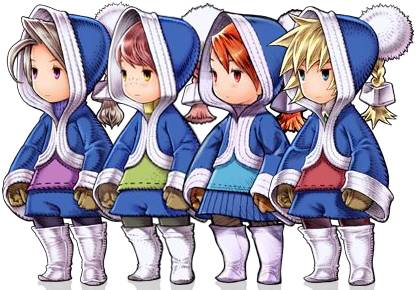
\includegraphics[width=\columnwidth]{./art/jobs/timemage.jpg}\ofrow
	\accf{Time Mages} are masters of time and space, who understand that imagination is more important than knowledge. 
	They manipulate the flow of time and bend the fabric of reality to their advantage. 
%	While Time Mages rarely fight on their own, they can decide an ongoing battle with their incredible abilities.
}
{Staff}{Robe}{
	Level 1: & HP~+17 & MP~+28 & AGI~+2 & MAG~+1 \\
	Level 2: & HP~+5  & MP~+10 & RES~+1 & STR~+1 \\
	Level 3: & \multicolumn{3}{l}{Archetype Attribute Bonus}  \\
	Level 4: & HP~+10  & MP~+10 & MAG~+1 &        \\ 
	Level 5: & HP~+10 & MP~+10 & RES~+1 &		  \\ 
	Level 6: & HP~+5  & MP~+10 & DEF~+1 & RES~+1 \\ 
	Level 7: & HP~+5  & MP~+10 & RES~+2 \\ 
	Level 8: & HP~+10  & MP~+10 & DEF~+1 \\ 
	Level 9: & HP~+5  & MP~+10 & RES~+2 &        \\ 
	Level 10:& HP~+5  & MP~+10 & MAG~+1 &	RES~+1	  
}{
	\ofjobspell{Gravity}{6}{0r}{Single}{3u}{The target suffers 2d damage and can only move half his usual distance on his next turn.}{}{1}\ofabilitygap
	\ofjobspell{Haste}{8}{0r}{Single}{5u}{The target gains Haste for 3 rounds.}{\haste}{2}\ofabilitygap
	\ofjobspell{Slow}{8}{0r}{Single}{5u}{The target suffers Slow for 3 rounds.}{\slow}{2}\ofabilitygap
	\ofjobspell{Float}{7}{0r}{Single}{3u}{The target levitates up to 3u above the ground for 3 rounds. While allies can still move in the air, targeted enemies suffer Immobile for the duration.}{}{4}\ofabilitygap
	\ofjobspell{Graviga}{15}{1r}{2u}{6u}{All enemies in the target area suffer 6d damage and a Slow Field appears in the target area that lasts for 3 rounds.}{}{6}\ofabilitygap
	\ofjobspell{Stop}{16}{0r}{30u}{Self}{All enemies in the target area make a DC 8 check and suffer Sleep for 1 round upon failure.}{\sleep}{8}\ofabilitygap
	\ofjobspell{Banish}{26}{0r}{Single}{5u}{Temporarily banish the target into another dimension. If he is an ally, he can still take turns, but not interact with the battlefield. After 3 rounds, the target reappears in the same spot, anyone in the same space is pushed aside and suffers 6d damage. You cannot use Banish consecutively on the same target or if a previous cast is still active.}{}{10}
}{
	\ofarchetypet{Illusionist}
	{HP~+5 & MP~+20 & MAG~+2}
	{\ofarchetypespella{Warp}{6}{0r}{1u}{5u}{You teleport to an unoccupied location of your choice that you can see within 5u.}{}}
	{\ofarchetypepassive{Tunneling}{Whenever you cast a spell, you can choose to double its range and target distance by also doubling its MP cost.}}
	{\ofarchetypereaction{Quick Warp}{Whenever you are targeted by an Attack, you can attempt to Warp. In this case, you make the evasion check with advantage and if you succeed, the Warp spell takes effect in addition to the evasion. In either case, you have to respect the spell's MP cost.}}
	{\ofarchetypespellb{Exchange}{14}{0r}{Single}{10u}{Choose two targets within range and exchange their positions. Targeted enemies suffer an additional 4d damage. Targeted allies instead cause 4d damage to everyone within 2u of their new position. Also, both targets push aside anything that would obstruct their new spot.}{}}
}{
	\ofarchetypet{Oracle}
	{HP~+8 & MP~+17 & STR~+1 & RES~+1}
	{\ofarchetypespella{Extend}{5}{0r}{Single}{5u}{The duration of all Status Effects that the target is suffering or benefiting from, is extended by 3 rounds.}{}}
	{\ofarchetypepassive{Read Ahead}{Right before the start of each combat, you can take one extra turn, even if the enemy has a surprise round.}}
	{\ofarchetypereaction{Kismet}{Whenever a spell or tech that targets someone within 5u takes effect, you can choose to delay it. In this case, the battle continues as usual and the ability instead takes effect on the target after 1 round.}}
	{\ofarchetypespellb{Quicken}{10}{0r}{Single}{5u}{The target takes an extra turn immediately before yours is finished. The round continues as usual afterwards, so you still have to pick the next combatant for your side. You can only use this ability once per round.}{}}
}
\thispagestyle{empty}
\subsection*{\huge Guerrero}
\vspace{0.3cm}
"Me da igual…". \\
\indent -- Squall 
\vspace{0.3cm} \\
Los Guerreros son especialistas en combate cuerpo a cuerpo debido a su poderosa capacidad física tanto en ataque como en defensa. Son expertos en el uso de espadas y armaduras, lo que les permite ser aún más peligrosos y resistentes. En su búsqueda de oponentes más fuertes, los Guerreros más experimentados saben que siempre hay un pez más gordo.
\vfill
\battrt{ \textbf{Nivel 1:} & PV~+25 & PM~+12 & AGI~+3 & FUE~+1 \\
 \textbf{Nivel 2:} & PV~+10 & PM~+5 & FUE~+1 & DEF~+1 \\
 \textbf{Nivel 3:} & PV~+10 & PM~+10 & RES~+1 &        \\
}{Espada}{Armadura Liviana, Armadura Pesada}
\vfill
\atypet{Caballero Oscuro} { \textbf{Nivel 4:} & PV~+5 & PM~+10 & FUE~+1 & RES~+1 \\ 
 \textbf{Nivel 5:} & PV~+10 & PM~+5 & DEF~+2 & 		  \\ 
 \textbf{Nivel 6:} & PV~+5 & PM~+10 & FUE~+2 &		  \\ 
 \textbf{Nivel 7:} & PV~+10 & PM~+5 & FUE~+1 & RES~+1 \\ 
 \textbf{Nivel 8:} & PV~+5 & PM~+5 & DEF~+1 & RES~+2 \\ 
 \textbf{Nivel 9:} & PV~+10 & PM~+5 & FUE~+1 & DEF~+1 \\ 
 \textbf{Nivel 10:}& PV~+10 & PM~+10 & RES~+1 &		  \\ 
} {Sacrificio} { Cuando hagas un \hyperlink{action}{Ataque} con éxito sobre un enemigo, puedes infligir daño \hyperlink{action}{Oscuro} equivalente a la mitad del daño original a ti y a todos los enemigos que se encuentren a ~3u. } {Precio de Sangre} { Siempre que un enemigo o un aliado (dispuesto) que se encuentre a 5u consuma PM, puedes obligarlo a que consuma sus PV en lugar de sus PM si tiene los suficientes PV para hacerlo. Luego, la mitad de ese valor se recupera a tus PV. }
\vfill
\atypet{Luchador} { \textbf{Nivel 4:} & PV~+10 & PM~+5 & FUE~+2 &        \\ 
 \textbf{Nivel 5:} & PV~+5 & PM~+10 & FUE~+1 & DEF~+1 \\ 
 \textbf{Nivel 6:} & PV~+10 & PM~+5 & DEF~+1 & RES~+1 \\ 
 \textbf{Nivel 7:} & PV~+5 & PM~+5 & FUE~+2 &        \\ 
 \textbf{Nivel 8:} & PV~+10 & PM~+5 & RES~+2 &        \\ 
 \textbf{Nivel 9:} & PV~+5 & PM~+10 & FUE~+1 & DEF~+1 \\ 
 \textbf{Nivel 10:}& PV~+10 & PM~+5 & DEF~+2 &        \\ 
} {Adrenalina} { Siempre que reduzcas los PV de un enemigo a 0, obtienes inmediatamente un turno extra. } {Punto Ciego} { Siempre que un enemigo en un radio de 1u inflija daño a un aliado o reciba daño de un aliado, inmediatamente puedes hacer un \hyperlink{action}{Ataque} sobre él. }
\pagebreak \\
\noindent {\Large\color{accent}\bf \uline{Habilidades\phantom{y}\hfill}}\\\\
\techt{Carga}{3}{0t}{Único}{Arma}{ Realiza un \hyperlink{action}{Ataque} contra el objetivo. Si lo golpeas, lo haces retroceder 1u además del daño infligido. }{}{1} \techt{Golpe Fuerte}{5}{0t}{Único}{Arma}{ Realiza un \hyperlink{action}{Ataque} en el que el objetivo tiene \hyperlink{check}{Ventaja} en la tirada de evasión. Si lo golpeas, haces \hyperlink{action}{Daño Crítico}. }{}{2} \techt{Rompearmadura}{10}{0t}{Único}{Arma}{ Realiza un \hyperlink{action}{Ataque} contra el objetivo. Si lo golpeas, el objetivo sufre \hyperlink{status}{disDEF} y \hyperlink{status}{disRES} por 3 turnos además del daño infligido. }{\dedef \deres}{3} \techt{Rompehuesos}{8}{0t}{Único}{Arma}{ Realiza un \hyperlink{action}{Ataque} contra el objetivo. Si lo golpeas, el objetivo queda \hyperlink{status}{Inmóvil} por 1 turno además del daño infligido. }{\immobile}{5} \techt{Enfocar}{6}{1t}{Objetivo}{Tú}{ Por los próximos 3 turnos, cada vez que realices un \hyperlink{action}{Ataque} sobre un enemigo, este tiene desventaja en la tirada de evasión. }{}{6} \techt{Valentía}{10}{1t}{2u}{Tú}{ Tú y todos los aliados que se encuentren en el área de efecto reciben \hyperlink{status}{aumFUE} y \hyperlink{status}{aumMAG} por 3 turnos. }{\enstr \enmag}{7} \techt{Vendaval}{8}{1t}{5u (línea)}{Tú}{ Realiza un \hyperlink{action}{Ataque} contra todos los que se encuentren en el área de efecto haciendo una sola tirada de daño que aplica a todos los afectados y que fallen la tirada de evasión. El daño infligido es de \hyperlink{type}{Viento}. }{\wind}{8} \techt{Andanada}{20}{1t}{5u}{Tú}{ Realiza un \hyperlink{action}{Ataque} contra todos los enemigos en el área de efecto haciendo una sola tirada de daño que aplica a todos los afectados y que fallen la tirada de evasión. Además, obtienes \hyperlink{status}{Reflejos} hasta el inicio de tu próximo turno. }{\blink}{9} \techt{Omnilátigo}{30}{0t}{Único}{Arma}{ Realiza 3 \hyperlink{action}{Ataques} separados contra el objetivo. Cada vez que el objetivo obtenga 4 o menos en la tirada de evasión, haces \hyperlink{action}{Daño Crítico}. }{}{10}
\pagebreak
\thispagestyle{empty}
\ofjob{White Mage}
{
	\ofquote{"Hey, that’s Cloud’s line! ’It’s too dangerous, I can’t get you involved...' Blah blah blah."\\}{Aerith}\\\\
	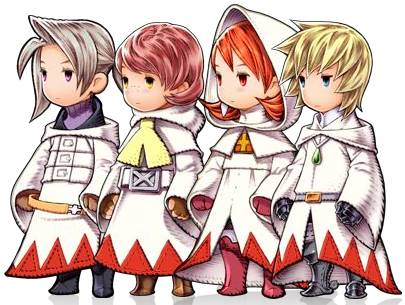
\includegraphics[width=\columnwidth]{./art/jobs/whitemage.jpg}\ofrow
	\accf{White mages} are experts of defensive magic and boast a variety of recovery and protective spells.
	While mediocre in physical combat, they also feature incredible resistance against magic. 
	Where others will succumb to the God of Death, a skilled White Mage will face him and say: "Not today".	
}
{Staff}{Robe}{
	Level 1: & HP~+19 & MP~+27 & AGI~+2 & RES~+1 \\
	Level 2: & HP~+5  & MP~+10 & MAG~+1 & STR~+1 \\
	Level 3: & \multicolumn{3}{l}{Archetype Attribute Bonus} \\
	Level 4: & HP~+10 & MP~+5 & MAG~+1 & DEF~+1	  \\
	Level 5: & HP~+5  & MP~+10 & RES~+1 &	STR~+1  \\ 
	Level 6: & HP~+5  & MP~+5 & MAG~+2 &        \\ 
	Level 7: & HP~+10  & MP~+10 & RES~+1 & DEF~+1 \\ 
	Level 8: & HP~+5 & MP~+5  & MAG~+2 & DEF~+1 \\ 
	Level 9: & HP~+5  & MP~+10 & RES~+1 &	MAG~+1   \\ 
	Level 10:& HP~+10 & MP~+10 & RES~+1 &	        
}{	
	\ofjobspell{Cure}{4}{0r}{Single}{3u}{The target regains 2d HP.}{}{1}\ofabilitygap
	\ofjobspell{Drain}{6}{0r}{Single}{4u}{Deal 1d damage to the target and increase your own HP by the total amount of damage dealt.}{}{2}\ofabilitygap
	\ofjobspell{Esuna}{6}{0r}{Single}{3u}{You remove all negative Status Effects except KO from the target.}{}{4}\ofabilitygap
	\ofjobspell{Curaga}{14}{1r}{2u}{5u}{Everyone in the target area regains 6d HP.}{}{6}\ofabilitygap
	\ofjobspell{Holy}{21}{2r}{Single}{7u}{You deal 6d+20 holy damage to the target.}{\holy}{8}\ofabilitygap
	\ofjobspell{Auto-Life}{28}{2r}{Single}{3u}{You summon a guardian angel that watches over the target. The next time he falls KO, he is instantly revived with 1 HP. This effect does not stack and if not activated, it expires when the target goes to sleep.}{\ko}{10}
}{
	\ofarchetypet{Sage}
	{HP~+11 & MP~+9 & MAG~+2 & STR~+1}
	{\ofarchetypespella{Sleep}{6}{0r}{Single}{3u}{The target makes a DC 8 check and suffers Sleep for 3 rounds upon failure.}{\sleep}
	\vspace*{0.1cm}\\ \ofarchetypespella{Silence}{6}{0r}{Single}{3u}{The target makes a DC 8 check and suffers Silence for 3 rounds upon failure.}{\silence}}
	{\ofarchetypepassive{Ancient Wisdom}{All magic damage that you deal ignores the RES of its targets. In addition, you can inflict Status Effects on targets that are Immune against them.}}
	{\ofarchetypereaction{Absorb MP}{When you are the target of an enemy ability, increase your MP by half the amount that the caster spent on it.}}
	{\ofarchetypespellb{Drainga}{18}{1r}{3u}{7u}{Deal 4d damage to all enemies in the target area and increase your HP by the total amount of damage dealt.}{}}
}{
	\ofarchetypet{Medic}
	{HP~+7 & MP~+13 & RES~+2 & DEF~+1}
	{\ofarchetypespella{Protect}{4}{0r}{Single}{5u}{The target gains EnDEF for 3 rounds.}{\enndef} \vspace*{0.1cm}\\ \ofarchetypespella{Shell}{4}{0r}{Single}{5u}{The target gains EnRES for 3 rounds.}{\enres}}
	{\ofarchetypepassive{Doctor's Code}{Whenever you use Magic on an ally within 1u, you can also immediately use an Item on him in addition.}}
	{\ofarchetypereaction{No Collateral}{Whenever you would be affected by a spell or tech that you are not the primary target of, you can choose that you and all other secondary targets are unaffected.}}
	{\ofarchetypespellb{Full-Life}{22}{2r}{Single}{5u}{Remove the KO status from the target and fully restore his HP.}{\ko}}
}

